% arara: pdflatex
% arara: biber
% arara: pdflatex
% arara: pdflatex if found('log', 'undefined references')
% \documentclass[draft,12pt,oneside,a4paper]{memoir}
\documentclass[12pt,article,oneside,a4paper]{memoir}


\usepackage[english]{babel}
\usepackage{graphicx}
\usepackage{subcaption}
\usepackage{amssymb}
\usepackage{amsmath}
\usepackage{amsthm}
\usepackage{bm}
\usepackage{multirow}
\usepackage[utf8]{inputenc}
\usepackage[style=english]{csquotes}
\usepackage{algorithm}
\usepackage[noend]{algpseudocode}
\usepackage{listings}
\usepackage{textcomp}
\usepackage{courier}
\usepackage{tikz}
\usepackage{datetime}
\usepackage{bibentry}
\usepackage[varg]{txfonts}
\usepackage{import}
\usepackage{tcolorbox}
\usepackage[backend=biber,
            bibstyle=numeric,
            citestyle=authoryear-comp,
            uniquelist=false,
            uniquename=false,
            sorting=nyt,
            url=false,
            maxcitenames=1,
            natbib=true,
            backref=true]{biblatex}

% Exclude \fullcite citation from bibliography
\DeclareBibliographyCategory{fullcited}
\newcommand{\mybibexclude}[1]{\addtocategory{fullcited}{#1}}


\usepackage[section]{placeins}
\usepackage[export]{adjustbox}
\lstset{language=Python,
  basicstyle=\ttfamily\bfseries\small,
  commentstyle=\color{red}\itshape,
  stringstyle=\ttfamily\color{green!50!black},
  showstringspaces=false,
  keywordstyle=\color{blue}\bfseries}%

\newcommand{\code}[1]{\lstinline{#1}}

% For the TODOs
\usepackage{xcolor}
\usepackage{xargs}
\usepackage[colorinlistoftodos,textsize=footnotesize]{todonotes}
\newcommand{\todoin}{\todo[inline]}
% from here: https://tex.stackexchange.com/questions/9796/how-to-add-todo-notes
\newcommandx{\unsure}[2][1=]{\todo[linecolor=red,backgroundcolor=red!25,bordercolor=red,#1]{#2}}
\newcommandx{\change}[2][1=]{\todo[linecolor=blue,backgroundcolor=blue!25,bordercolor=blue,#1]{#2}}
\newcommandx{\info}[2][1=]{\todo[linecolor=OliveGreen,backgroundcolor=OliveGreen!25,bordercolor=OliveGreen,#1]{#2}}

% \usepackage{microtype}
\usepackage[activate={true,nocompatibility},%
final,tracking=true,kerning=true,spacing=true,%
factor=1100,stretch=10,shrink=10]{microtype}

\usepackage{tcolorbox}
\usepackage{newtxmath}
\usepackage[plainpages=false,
            pdfpagelabels,
            bookmarksnumbered,
            draft=false,
            colorlinks,
            ]{hyperref}
\usepackage{cleveref}
\usepackage{newtxmath}
\usepackage{titling}
% \usepackage[displaymath,mathlines]{lineno}

\definecolor{linkcolour}{rgb}{0,0.2,0.6}
\definecolor{citecolour}{rgb}{0,0.6,0.2}
\definecolor{urlcolour} {rgb}{0.8,0,0.8}

\hypersetup{%
  pdftitle={Coupled Smoothed Particle Hydrodynamics--Discrete Element Method
    for Fluid and Solid Mechanics},
  pdfauthor={Dinesh Adepu},
  linkcolor=linkcolour,citecolor=citecolour,
  filecolor=urlcolour,urlcolor=urlcolour, }


%% IITB Thesis guidelines
\renewcommand{\rmdefault}{ptm}

%%%% use Latin Modern for other fonts
% \renewcommand{\sfdefault}{lmss}
% \renewcommand{\ttdefault}{lmtt}


%%% set up the page layout
\settrimmedsize{11in}{210mm}{*}
\setlength{\trimtop}{0pt}
\setlength{\trimedge}{\stockwidth}
\addtolength{\trimedge}{-\paperwidth}
\settypeblocksize{7.75in}{33pc}{*}
% \setulmargins{4cm}{*}{*}
% \setlrmargins{1.5in}{*}{*}
% IITB Margins
\setlrmarginsandblock{3cm}{2cm}{*}
\setulmarginsandblock{3.8cm}{3.5cm}{*}

\setmarginnotes{17pt}{51pt}{\onelineskip}
\setheadfoot{\onelineskip}{2\onelineskip}
\setheaderspaces{*}{2\onelineskip}{*}
\setsidefeet{\marginparsep}{9em}%
   {\onelineskip}{0pt}%
   {\normalfont\footnotesize}{\textheight}%
\settypeoutlayoutunit{cm}
\checkandfixthelayout%

\crefname{section}{Section}{Sections}

\newlength\figureheight%
\newlength\figurewidth%

\preto\fullcite{\AtNextCite{\defcounter{maxnames}{99}}}

%%% Macro definitions for Commonly used symbols
\newcommand{\ten}[1]{\ensuremath{\mathbf{#1}}}
\newcommand{\vb}[1]{\ensuremath{\mathbf{#1}}}
\newcommand{\grad}{\ensuremath{\nabla}}
\newcommand{\proj}{\ensuremath{\mathcal{P}}}
\newcommand{\divergence}{\ensuremath{\nabla \cdot}}
\newcommand{\divt}{\ensuremath{\mathop{\text{div}}}}
\newcommand{\interval}{\ensuremath{\mathop{\text{I}}}}
\newcommand{\gradt}{\ensuremath{\mathop{\text{grad}}}}
\newcommand{\mathtext}[1]{\ensuremath{\mathop{\text{#1}}}}
\newcommand{\qqtext}[1]{\ensuremath{\quad \text{#1} \quad}}
\newcommand{\qin}{\ensuremath{\quad \text{in} \quad}}
\newcommand{\qand}{\ensuremath{\quad \text{and} \quad}}
\newcommand{\qon}{\ensuremath{\quad \text{on} \quad}}
\newcommand{\laplacian}{\ensuremath{\nabla^2}}
\newcommand{\teng}[1]{\ensuremath{\boldsymbol{#1}}}
\newcommand{\Rey}{\operatorname{\mathit{R\kern-.04em e}}}

\theoremstyle{definition}
\newtheorem*{remark}{Remark}
% Change font size to conform with the rest of the document text
\renewcommand{\abstracttextfont}{\normalsize}
\renewenvironment{abstract}{\chapter*{\abstractname}}{}


\newdateformat{monthyeardate}{\large\monthname[\THEMONTH], \THEYEAR}
\newdateformat{yeardate}{\large \THEYEAR}

\addbibresource[datatype=bibtex]{mylit.bib}
\urlstyle{tt}
\emergencystretch=1em

\DeclareSourcemap{
  \maps[datatype=bibtex]{
    \map{
      \step[fieldsource=url,final]
      \step[fieldset=doi,null]
    }
  }
}
\renewcommand*{\nameyeardelim}{\addspace}
\newcommand{\Usefont}[1]{\fontfamily{#1}\selectfont}
\newcommand{\putiitblogo}{
\includegraphics[width=10em]{iitb-black}}
\newcommand{\reporttype}{
  \textit{Proposed to be submitted in}\\
  \emph{Partial fulfilment of the requirements for the Degree of}\vskip2.0\baselineskip%
  {\large Doctor of Philosophy}\vskip2.0\baselineskip%
  \textit{of the}\vskip2.0\baselineskip%
  INDIAN INSTITUTE OF TECHNOLOGY BOMBAY\vskip2.0\baselineskip%
 \textit{by}\vskip2.0\baselineskip%
}

\makeatletter
\newcommand*{\titleGM}{%
\thispagestyle{empty}
\begin{center}
\begingroup% Gentle Madness
\hbox{%
    \vbox{%
      {\bfseries INDIAN INSTITUTE OF TECHNOLOGY BOMBAY\par}
      {Department of Aerospace Engineering\par}\vskip2.0\baselineskip%
      \textit{SYNOPSIS}\vskip2.0\baselineskip%
      \textit{of the Ph.D. thesis entitled}\vskip2.0\baselineskip%
      {\Large\bfseries\@title\par}\vskip2.0\baselineskip%
      {\reporttype\par}%
      {\@author\par}
      \vspace{2\baselineskip}
      {\@date\par}
    }% end of vbox
  }% end of hbox
\vfill%
\null%
\endgroup
\end{center}
}
\makeatother

\newbox\keywbox
\setbox\keywbox=\hbox{\bfseries Keywords:}%
\newcommand\keywords{\noindent\rule{\wd\keywbox}{0.25pt}\\\textbf{Keywords:}\ }


\begin{document}


\title{Coupled Smoothed Particle Hydrodynamics-Discrete Element Method for
  Fluid and Solid Mechanics} \author{%
  {\Large Dinesh Adepu} \\
  \normalfont{Roll No. 153010009} \\
  \vspace{0.2cm}
  \normalfont{Supervisor:} \\
  {\large Prof.\ Prabhu Ramachandran} }

\monthyeardate{}

% \degree{M.Tech.~$+$~Ph.D. Dual Degree}
% \dept{Department of Aerospace Engineering}

\titleGM%
\thispagestyle{empty}

\frontmatter%
% Use make subsections appear in the contents. Use numdepth to make numbering
% appear as well.
\settocdepth{subsection}


\setlength{\unitlength}{1pt}

\begingroup
% important point here: We need \endlineshar=-1 here for the inline
% list of subsections. Why? Beacause we have subsection subsubsection
% subsection, and under hyperref running the l@subsubsection for
% subsubsection, which typesets nothing, ruins our \ignorespaces in
% our redefinition of \l@subsection (it cannot see and ignore the space after the
% \contentsline line for subsubsection). Easiest solution: use
% change \endlinechar
%
% Special thanks to David Carlisle in the tex.stackexchange.com chat
% for suggesting it

\endlinechar=-1

\endgroup

\chapterstyle{article}
% \counterwithout{section}{chapter}
\epigraphfontsize{\small\itshape}%
\setlength\epigraphwidth{.8\textwidth}
\setlength\epigraphrule{0pt}


% \pagestyle{simple}
% Center the page numbers
\copypagestyle{mine}{ruled}
\makeevenfoot{mine}{}{\thepage}{}
\makeoddfoot{mine}{}{\thepage}{}
\pagestyle{mine}


\mainmatter%
\setsecnumdepth{subsubsection}

\chapter{Introduction}
\label{chap:intro}
Several real-life applications involve fluid dynamics, structural dynamics, and
interaction between these two materials. Examples include fluid-structure
interaction, rigid body collision inside fluid flow, rigid bodies colliding,
\begin{figure}[!htpb]
  \centering
  \includegraphics[width=0.7\textwidth]{images/intro/images/intro_section/erosion_hand_drawn_2}
  \caption{A schematic of erosion of a ductile solid due to several arbitrarily
    shaped solids impacting it in a fluid flow.}
\label{fig:intro-big-picture}
\end{figure}
deforming, and eroding an elastic-plastic target. \Cref{fig:intro-big-picture}
depicts a complex physical process. From \Cref{fig:intro-big-picture}, we can
see the erosion of a ductile solid due to the impact of rigid bodies in a fluid
flow. From the numbered labels, one needs to model the following physics to
model a problem such as this,
\begin{enumerate}
\item fluid dynamics,
\item elastic-plastic dynamics,
\item fluid-structure interaction (FSI),
\item free rigid body dynamics,
\item rigid-fluid coupling (RFC) and rigid-rigid interaction and,
\item solid particle erosion (SPE).
\end{enumerate}
We employ particle-based numerical methods to model the physical processes
involved in handling a problems like in \cref{fig:intro-big-picture}, due to the
natural ability to handle free surfaces and large deformation problems. We use a coupled
smoothed particle hydrodynamics (SPH) and discrete element method (DEM)
formulation to model the physical processes. We now review the state of the art
in SPH and DEM to model these physical processes.


To model fluid and elastic dynamics, we choose SPH. SPH method has been
extensively applied to fluids, elastic dynamics, fluid-structure interaction
among other areas~\parencite{monaghan2012smoothed}. Due to its meshless and
Lagrangian nature the particles move with the local velocity and can introduce
disorder in the particles and thereby significantly reduce the accuracy of the
method. To ensures particle homogenization, \textcite{Adami2013} proposed
Transport Velocity Formulation (TVF) in SPH and applied to internal flow
problems, producing very accurate results. A generalized TVF by
\textcite{zhang_hu_adams17} is proposed to simulate free surface flow problems.
However, \textcite{Adami2013,zhang_hu_adams17} do not consider additional terms
while recasting the governing equations to the transport velocity formulation.
Further, GTVF leads to tensile instability in solids, when used with a different
PST.


In modeling the collision of elastic solids, SPH has been successful
\parencite{gray2001sph}. However, it does not consider friction between the
colliding solids. Another problem is that the model generates spurious forces on
bodies which are moving close to each other. \textcite{yan2021simulation}
introduced the interfacial SPH scheme, which eliminates the spurious
interactions but it cannot handle friction between the solids. Additionally the
interaction force does not consider the shape of the solids in contact.


FSI is modeled by several works using SPH, such as, weakly compressible
SPH-Total Lagrangian SPH (TLSPH), WCSPH-Updated Lagrangian SPH (ULSPH),
incompressible SPH-TLSPH~\parencite{khayyer2022systematic}. However, no work is
reported in an updated Lagrangian framework to model FSI with a transport
velocity formulation with corrections included.


In order to simulate rigid-rigid interaction between the bodies with irregular
geometries multi-sphere approach \parencite{kruggel-emden_study_2008}, and
surface mesh represented (SMR)-DEM ~\parencite{zhan2021surface} are used.
However, the multi-sphere approach fails to handle the contact accurately with
bodies involving sharp corners, as the force law assumes the contact between two
spherical particles. SMR-DEM requires additional information to handle the
collision, such as connectivity between the particles comprising the body in
addition to the particle positions. Additionally, we need additional sets of
particles to handle the interaction between the rigid body and the fluid
particles to model rigid-fluid coupling.


To simulate solid particle erosion, \textcite{dong2016smoothed} uses smoothed
particle hydrodynamics (SPH). However, \textcite{dong2016smoothed} does not
consider the arbitrary shape of the projectile. Further, collision among the
projectiles while interacting with the target is not modeled. To the authors
knowledge there is no open-source implementation in the literature which can
model the solid particle erosion using SPH.


Having discussed the drawbacks in modeling of these complex physical processes,
in the current work we develop an open-source framework to model the complex
physics. The following are the key goals of the work.
\begin{itemize}
\item Develop a unified technique in SPH to solve both fluid and solid dynamics
  problems.
\item Handle the collision between the elastic solids using a penalty-based contact force.
\item Handle the collision among the arbitrarily shaped rigid projectiles in fluid
  flow. Solve the two-way coupling between the fluid and the rigid bodies.
\item Develop a fluid-structure interaction solver.
\item Provide an open-source implementation for solid particle erosion in SPH.
\end{itemize}

We propose a corrected transport velocity formulation (CTVF) which works for both
solid mechanics and fluid mechanics problems. We study the importance of the
missing terms while recasting the governing equation to transport velocity
formulation. We employ the EDAC formulation to the transport velocity
formulation and show that there are additional correction terms in the EDAC
scheme that should be introduced to improve the accuracy of the method. The
method is also robust to the choice of the smoothing kernel.

We model the collision between elastic solids using a penalty-based contact
force model. The penalty-based force considered here is the one proposed by
\textcite{mohseni2021particle}. We explore the importance of choosing the
primary and secondary body under collision. We also eliminate the spurious
interaction forces between nearby interacting bodies and show how the contact
force can be used for elastic bodies. Additionally, friction between the
colliding solids is considered with the current formulation.

We model FSI problems with the CTVF method. We model both fluids and solid
material using CTVF alone. We couple CTVF with DEM to model the rigid fluid
coupling problems. The fluid phase is handled using the CTVF, which provides
smooth pressure distribution with EDAC formulation. DEM is used to handle
rigid-rigid interactions The interaction between the fluid phase and rigid
bodies is handled using the dummy particle approach \parencite{Adami2012}.

We develop a framework to model the solid particle erosion with CTVF method to
model the elastic-plastic behavior of the ductile target. The plastic
behavior is incorporated using a Johson-Cook constitutive model. The interaction
between the arbitrarily shaped solids and the ductile target are modeled with a
modified contact force formulation. We establish the framework such that it can
handle erosion due to multiple impacts. Here, we allow the multiple particles to
also interact among themselves.



In the next few sections we give an overview of the our work in modeling these
physical processes.

\FloatBarrier%
\chapter{Numerical modeling of fluid and elastic dynamics}
\label{chap:ctvf}

\begin{equation}
  \label{eq:ce}
  \frac{d \rho}{d t} = - \rho \; \frac{\partial u_i}{\partial x_i},
\end{equation}
and conservation of linear momentum,
\begin{equation}
  \label{eq:me}
  \frac{d u_i}{d t} = \frac{1}{\rho} \; \frac{\partial \sigma_{ij}}{\partial x_j}
  + g_i,
\end{equation}

where $\rho$ is the density, $u_i$ is the $i$\textsuperscript{th} component of
the velocity field, $x_j$ is the $j$\textsuperscript{th} component of the
position vector, $g_i$ is the component of body force per unit mass and
$\sigma_{ij}$ is stress tensor.


The stress tensor is split into isotropic and deviatoric parts,
\begin{equation}
  \label{eq:stress_tensor_decomposition}
  \sigma_{ij} = - p \; \delta_{ij} + \sigma'_{ij},
\end{equation}
%
where $p$ is the pressure, $\delta_{ij}$ is the Kronecker delta function, and
$\sigma'_{ij}$ is the deviatoric stress.

The Jaumann's formulation for Hooke's stress provides us with the rate of
change of deviatoric stress,
\begin{equation}
  \label{eq:jaumann-stress-rate}
  \frac{d \sigma'_{ij}}{dt} = 2G (\dot{\epsilon}_{ij} - \frac{1}{3}
  \dot{\epsilon}_{kk} \delta_{ij}) + \sigma^{'}_{ik}  \Omega_{jk} +
  \Omega_{ik} \sigma^{'}_{kj},
\end{equation}
where $G$ is the shear modulus, $\dot{\epsilon}_{ij}$ is the strain rate tensor,
\begin{equation}
  \label{eq:strain-tensor}
  \dot{\epsilon}_{ij} = \frac{1}{2} \bigg(\frac{\partial u_i}{\partial x_j} +
  \frac{\partial u_j}{\partial x_i} \bigg),
\end{equation}
and $\Omega_{ij}$ is the rotation tensor,
\begin{equation}
  \label{eq:rotational-tensor}
  \Omega_{ij} = \frac{1}{2} \bigg(\frac{\partial u_i}{\partial x_j} -
  \frac{\partial u_j}{\partial x_i} \bigg).
\end{equation}

For a weakly-compressible or incompressible fluid, a viscous force is added:
\begin{equation}
  \label{eq:fluid-stress-decomposition}
  \sigma_{ij} = - p \delta_{ij} + 2 \eta \frac{\partial u_i}{\partial x_j}
\end{equation}
where $\eta$ is the kinematic viscosity of the fluid.

In both fluid and solid modelling the pressure is computed using an
isothermal equation of state, given as,
\begin{equation}
  \label{eq:pressure-equation}
  p = K \bigg(\frac{\rho}{\rho_{0}} - 1 \bigg),
\end{equation}
where $K = \rho_{0} c_0^2$ is the bulk modulus. Here, the constants $c_0$ and
$\rho_0$ are the reference speed of sound and density, respectively. For solids,
$c_0$ is computed as $\sqrt{\frac{E}{3 (1 - 2 \nu)\rho_{0}}}$, $\nu$ is the
Poisson ratio, $E$ is the Young's modulus.

\section{Numerical method}
In CTVF we move the particles with a \emph{transport velocity},
$\tilde{\ten{u}}$. The material derivative in this case is written as,
\begin{equation}
  \label{eq:modified-material-derivative}
  \frac{\tilde{d} }{d t} = \frac{\partial }{\partial t} +
  \tilde{u}_j \frac{\partial }{\partial x_j}.
\end{equation}

We therefore recast the governing equations to incorporate the transport
velocity. The new governing equations are,
\begin{equation}
  \label{eq:ce-tvf}
  \frac{\tilde{d} \rho}{d t} =
  - \rho \frac{\partial \tilde{u}_j}{\partial x_j} +
  \frac{\partial (\rho (\tilde{u}_j - u_j))}{\partial x_j}.
\end{equation}
We therefore write the momentum equation as,
\begin{equation}
  \label{eq:mom-tvf}
  \frac{\tilde{d} u_i}{d t} =
  \frac{\partial}{\partial x_j} (u_i (\tilde{u}_j - u_j))
  - u_i \frac{\partial}{\partial x_j} (\tilde{u}_j - u_j)
  + g_i
  +\frac{1}{\rho} \frac{\partial \sigma_{ij}}{\partial x_j}.
\end{equation}
We note that this equation encompasses both fluid dynamics as well as elastic
dynamics by simply changing the way $\sigma_{ij}$ is modeled. The first term
on the right-hand-side of \cref{eq:mom-tvf} is the additional artificial
stress term that is included in the TVF~\citep{Adami2013}. The second term
involves the divergence of the transport velocity field. In the case of the
TVF, the term includes a background pressure acceleration that is of the form,
\begin{equation}
  \label{eq:tvf-accel}
  \bigg(\frac{d \ten{u}_a}{dt}\bigg)_{c} = - p^0_a \sum_{b \in N(a)}
  \frac{m_b}{\rho_b^2} \nabla W(\ten{r}_{ab}, \tilde{h}_{ab}),
\end{equation}
where $p^0_a$ is the background pressure for the given particle $a$,
$\ten{r}_{ab} = \ten{r}_a - \ten{r}_b$, $\tilde{h}_{ab} = (h_a + h_b)/2$, and
index $b$ refers to the neighbors of particle $a$. The additional terms arising
while adjusting the continuity and momentum to the transport velocity are
certainly not zero and therefore this should not be ignored. We investigate the
importance of including these terms in \cref{sec:results}. We note that in the
case of elastic dynamics that these terms are negligible and do not make a
significant difference. This has also been pointed out by
\cite{zhang_hu_adams17}.

The Jaumann stress rate is also similarly modified to account for the
transport velocity as,
\begin{multline}
  \label{eq:modified-jaumann-stress-rate}
  \frac{\tilde{d} \sigma'_{ij}}{dt} = 2G (\dot{\epsilon}_{ij} - \frac{1}{3}
  \dot{\epsilon}_{kk} \delta_{ij}) + \sigma^{'}_{ik}  \Omega_{jk} +
  \Omega_{ik} \sigma^{'}_{kj} + \\
  \frac{\partial}{\partial x_k}\big(\sigma^{'}_{ij}  (\tilde{u}_k - u_k)\big)
  - \sigma^{'}_{ij} \frac{\partial}{\partial x_k} (\tilde{u}_k - u_k).
\end{multline}


The original EDAC-SPH ~\citep{edac-sph:cf:2019} scheme adjusted to
the transport velocity written as,
\begin{equation}
  \label{eq:edac-p-evolve}
  \frac{\tilde{d} p}{d t} =
  (p -\rho c_s^2)
    \text{div}(\ten{u})
  - p \; \text{div}(\tilde{\ten{u}})
    + \text{div}(p (\tilde{\ten{u}} - \ten{u}))
    + \nu_{edac}  \nabla^2 p.
\end{equation}
where $\nu_{edac}$ is a viscosity parameter for the smoothing of the pressure
and $c_s$ is the (artificial) speed of sound.
%
The value of $\nu_{edac}$ is,
\begin{equation}
  \label{eq:nu-edac}
  \nu_{edac} = \frac{\alpha_{\textrm{edac}} h c_s}{8},
\end{equation}
where $h$ is the smoothing length of the kernel and a value of
$\alpha_{\textrm{edac}}=0.5$ is recommended as suggested in~\citep{PRKP:edac-sph-iccm2015}.


\FloatBarrier%
\subsection{Lid driven cavity}
\label{sec:ldc}

We evaluate the ability of the proposed scheme to handle solid wall boundary
conditions by simulating a lid-driven cavity. The lid-driven cavity is a
classic problem that can be challenging to simulate in the context of the SPH.
It has been simulated by \citep{Adami2013}, \citep{huang_kernel_2019},
\citep{edac-sph:cf:2019} to note a few. A rectangular cavity with length 1 m
which is filled with fluid is constrained by four walls. Top wall has a
velocity of $U = 1 $ m\,s\textsuperscript{-1}. A unit density is assumed for the
fluid. The speed of sound of the fluid particle is set to $c = 10 U_{max}$. We
use the summation density to compute the density. The viscosity of the fluid
is set through the Reynolds number of the flow, $\nu = \frac{Re}{U}$. No
artificial viscosity is used in the current problem.

%
\begin{figure}
  \centering
  \includegraphics[width=0.5\linewidth]{figures/ctvf/figures/cavity/uv_re100}
  \caption{Velocity profiles $u$ vs.\ $y$ and $v$ vs.\ $x$ for the
    lid-driven-cavity problem at $Re=100$ with three initial particle
    arrangement of $50 \times 50$, $100 \times 100$, and $150 \times
    150$.}%
  \label{fig:ldc:uv_re100}
\end{figure}
%
\begin{figure}
  \centering
  \includegraphics[width=0.5\linewidth]{figures/ctvf/figures/cavity/uv_re1000}
  \caption{Velocity profiles for the lid-driven-cavity using the steady state
    simulation procedure for $Re = 1000$ with initial partial arrangement of
    $50 \times 50$, $100 \times 100$, and $200 \times 200$ compared with
    the results of~\citep{ldc:ghia-1982}.}%
\label{fig:ldc:uv_re1000}
\end{figure}

We now study convergence of the method as we vary the
resolution. \Cref{fig:ldc:uv_re100} and \cref{fig:ldc:uv_re1000} show the
center-line velocities $u$ versus $y$ and $v$ versus $x$ for the Reynolds
numbers 100 and 1000 respectively. For the $Re=100$ case we use three
different resolutions of $50\times 50, 100 \times 100$ and $150 \times
150$. For the $Re=1000$ case, we use an initial $50 \times 50$,
$100 \times 100$, and $200 \times 200$ grid of particles. These are compared
against the results of \citep{ldc:ghia-1982}. As we can see that the current
scheme is able to predict the velocity profiles well.


\FloatBarrier%
\subsection{Oscillating plate}
\label{sec:oscillating-plate}
We consider a thin oscillating plate that is clamped on one side.
An oscillating plate with a length of $0.2$ m and a height of $0.02$ m is
initially given with a velocity profile of,
%
\begin{equation*}
  v_y(x) = V_f \, c_0 \frac{F(x)}{F(L)},
\end{equation*}
where $V_f$ varies for different cases. $L$ is the length of the plate. $F(x)$
is given by,
\begin{multline}
  F(x) = (\cos(kL) + \cosh(kL)) \, (\cosh(kx) - \cos(kx)) + \\
  (\sin(kL) - \sinh(kL)) \, (\sinh(kx) - \sin(kx)).
\end{multline}
%
In the present example $kL$ is 1.875. The material properties of the plate are
as follows, Young's modulus $E=2.0\times 10^6$ Pa, a Poisson's ratio of
$\nu=0.3975$. $c_0$ is speed of sound, and a density of $\rho=1000$
kg\,m\textsuperscript{-3}, as done in~\citep{gray-ed-2001}.  In all the cases
simulated here, we use an $\alpha$ of $1$ for artificial viscosity.

This is further demonstrated by a case where an oscillating plate of length of
$0.2$ m and a height of $0.02$ m is simulated for a time of $0.22$ seconds.
Similarly, another case where plate of height $0.01$ m and a width of $0.2$ m is
run for a time of $0.51$ s.
\Cref{fig:oscillating-plate:etvf-sun2019-l-0-2-h-0-22} and
\cref{fig:oscillating-plate:etvf-sun2019-l-0-2-h-0-01} shows particles of the
plate at time $t=0.22$ s and $0.51$ s of these two cases respectively. As we can
see from the figure that the plate is free of numerical fracture, thus the
tensile instability is eliminated.
%
%
\begin{figure}
  \centering
  \includegraphics[width=0.8\columnwidth]{figures/ctvf/figures/oscillating_plate/etvf_sun2019_l_0_2_h_0_02}
  \caption{Oscillating plate at time $t=0.22$s with a length of $0.2$m and
    height of $0.02$m simulated with SPST with CTVF scheme.}
\label{fig:oscillating-plate:etvf-sun2019-l-0-2-h-0-22}
\end{figure}
%
%
\begin{figure}[!htp]
  \centering
  \includegraphics[width=0.8\columnwidth]{figures/ctvf/figures/oscillating_plate/etvf_sun2019_l_0_2_h_0_01}
  \caption{Oscillating plate at time $t=0.51$s with a length of $0.2$m and
    height of $0.01$m simulated with SPST with CTVF scheme.}
\label{fig:oscillating-plate:etvf-sun2019-l-0-2-h-0-01}
\end{figure}

The accuracy of the current scheme is evaluated by comparing with the
analytical results and with a convergence study. In
\cref{table:compare-analytical-with-simulated-h-l-0-1} we compare the time
period for the oscillation by the analytical and the numerical results with
varying $V_f$, where we consider an oscillating plate whose $H/L$ ratio is
$0.1$. The difference between the analytical result and the numerical result
is due to the fact that the analytical results are based on thin plate theory
where as the plate considered here has a finite thickness. Further, we can see
that the current numerical results are in agreement with the previously
reported numerical results~\citep{gray-ed-2001, zhang_hu_adams17}. In
\cref{fig:oscillating:ipst_convergence_plot}, we have performed a convergence
study of an oscillating plate, with a $\nu=0.3975$, and $V_f=0.05$
m\,s\textsuperscript{-1}, and IPST is used for particle homogenization. The trend of
the current scheme matches well with the other updated Lagrangian SPH
schemes~\citep{gray-ed-2001, zhang_hu_adams17}. Hence the current scheme is
able to work with different PST methods and removes the tensile instability.

\begin{table}[!htpb]
\centering
\begin{tabular}{c c c c c}
  \hline
  $V_f$ & 0.001 & 0.01 & 0.03 & 0.05 \\
  \hline
  $\text{T}_{\mathrm{CTVF}}$ & 0.284 & 0.283 & 0.283 & 0.284 \\
  $\text{T}_{\mathrm{GTVF}}$ & 0.284 & 0.283 & 0.284 & 0.285 \\
  $\text{T}_{\mathrm{analytical}}$ & 0.254 & 0.252 & 0.254 & 0.254
\end{tabular}
\caption{Comparison between the CTVF and the analytical solution for the time
  period of the oscillating plate with a length of $0.2$m and height of
  $0.02$m with various $V_f$}
\label{table:compare-analytical-with-simulated-h-l-0-1}
\end{table}

\FloatBarrier%
\chapter{CSPH}
\label{chap:csph}

We model the collision between elastic solids using a penalty-based contact
force model. A contact force based approach for collision handling will
eliminate the spurious interaction between bodies, which occurs while modeling
with an SPH-based model. The contact force model follows the work of
\textcite{mohseni2021particle}.

The governing equations of including the new contact force term are:
\begin{equation}
\label{eqn:sph-continuity}
  \frac{\tilde{d}\rho_a}{dt} = \sum_{b \in A} \; \frac{m_b}{\rho_{b}} \; (
  \rho_{a} \; \tilde{\ten{u}}_{ab} \; + \;
  (\rho \; (\tilde{\ten{u}} \; - \;
  \ten{u}))_{ab}) \; \cdot \nabla_{a} W_{ab},
\end{equation}
\begin{equation}
\label{eqn:sph-momentum}
  \frac{\tilde{d}\ten{u}_{a}}{dt} = - \sum_{b \in A} m_b \bigg[
  \bigg(\frac{p_a}{\rho_a^2} + \frac{p_b}{\rho_b^2}\bigg) \ten{I} -
  \bigg(\frac{\teng{\sigma}^{'}_{a}}{\rho_a^2} +
  \frac{\teng{\sigma}^{'}_{b}}{\rho_b^2} + \Pi_{ab} \ten{I} \bigg) \bigg]  \cdot \nabla_{a} W_{ab} +
  \ten{g}_{a} + \frac{1}{m_a}\sum_{b \in B} \ten{F}^{\text{cont}}_{a \leftarrow b}.
\end{equation}
Here, $\ten{F}^{cont}_{a}$ is the force acting on particle $a$ due to
\begin{figure}[!htpb]
  \centering
  \includegraphics[width=1.0\textwidth]{images/csph/images/contact_force/contact_force_description}
  \caption{Bodies under collision which are divided into primary and
    secondary.}
\label{fig:bodies_under_collision}
\end{figure}
contact with the other elastic bodies.

The contact force $\ten{F}^{cont}_{a}$ is computed using
\textcite{mohseni2021particle} formulation. The force acting on a particle $a$ of
body A due to the interaction with the particles of body $B$ is into a normal
and tangential component. The normal force ($\teng{F}_a^{n}$) on particle $a$
due to the interaction with the particles $b$ of body $B$ is computed as,
\begin{equation}
  \label{eq:contact-algorithm-normal}
  \ten{F}_a^n = k_r \delta_{n^{c}}^{a} \ten{n}_a^{c}.
\end{equation}
Here, the overlap $\delta_{n^{c}}^{a}$ is a normal vector, and
$\delta_{n^{c}}^{a}$ is an overlap which is computed using a smoothed distance
formulation to handle arbitrarily shaped solids.

Tangential component of the contact force is computed by associating a
tangential spring attached to particle $a$ ($|\Delta \textit{\textbf{l}}_a|$)
and body $B$, which is initiated to a magnitude of zero
($|\Delta \textit{\textbf{l}}_a|=0$). The tangential spring is activated when
the particle comes into contact with body $B$. The tangential force is coupled
to the normal force through the Coulomb's law,
\begin{equation}
  \label{eq:Coulomb-law}
  \ten{F}_{a}^{t} = \min(\mu |\ten{F}_{a}^{n}|, |\ten{F}_{a}^{t}|) \
  \frac{\ten{F}_{a}^{t}}{|\ten{F}_{a}^{t}|}.
\end{equation}
This allows us to impose the sliding friction condition between the
interacting solids. Finally, the total force acting on the particle $a$ due to
the interaction with body $B$ is:
\begin{equation}
  \label{eq:contact-force}
  \ten{F}_{a}^{\text{cont}} = \ten{F}_{a}^{n} + \ten{F}_{a}^{t}
\end{equation}

\begin{figure}[!htpb]
  \centering
  \includegraphics[width=0.3\textwidth]{images/csph/images/contact_force/contact_force_description_3}
  \caption{Force transfer to the secondary particles $b$ from the primary body particle $a$}
\label{fig:secondary_particle_contact_foce_transfer}
\end{figure}
An equal and opposite force of the same magnitude is applied to the closest
secondary particle $b$ of $a$ as shown in
\cref{fig:secondary_particle_contact_foce_transfer},
\begin{equation}
  \label{eq:contact-force}
  \ten{F}_{b}^{\text{cont}} = - \ten{F}_{a}^{\text{cont}}.
\end{equation}

% =========================================== %
% ------ Results start ---------------------- %
% =========================================== %

\FloatBarrier%
\section{Stress wave propagation in granular media}
\label{sec:results-stress-wave-propagation-with-friction}
% \begin{figure}[!htpb]
%   \centering
%   \includegraphics[width=1.0\textwidth]{images/csph/images/de_2021_stress_wave_in_granular_material_part_2/schematic}
%   \caption{Schematic of the initial placement of the frictional granular media including the impactor and walls}
% \label{fig:results-stress-wave-propagation-part-II}
% \end{figure}
We demonstrate current solver abilities in handling the collision between the
multiple elastic solids by simulating the elastic wave propagation in a granular
media. We consider five identical disks placed at an angle of $45$ degrees,
allowed to be impacted by a moving wall from right with a velocity $5.6$
m\,s\textsuperscript{-1} in horizontal direction.
\Cref{fig:de-stress-wave-compare} shows the particle plots of the granular discs
with the stress fringes from the experiment \citep{guilkey2001improved}, and the
simulation carried in the present study, and from the numerical study of
\textcite{de2021modelling}, where the simulation is carried out using a total
Lagrangian material point method (TLMPM).
\begin{figure}[!htpb]
  \centering
  \begin{subfigure}{1.0\textwidth}
    \centering
    \includegraphics[width=0.7\textwidth]{images/csph/images/de_2021_stress_wave_in_granular_material_part_2/bardenhagen_2001}
    \subcaption{}\label{fig:de-stress-wave-bardenhagen}
  \end{subfigure}

  \begin{subfigure}{1.0\textwidth}
    \centering
    \includegraphics[width=0.7\textwidth]{images/csph/images/de_2021_stress_wave_in_granular_material_part_2/tlmpm_2021}
    \subcaption{}\label{}
  \end{subfigure}

  \begin{subfigure}{1.0\textwidth}
    \centering
    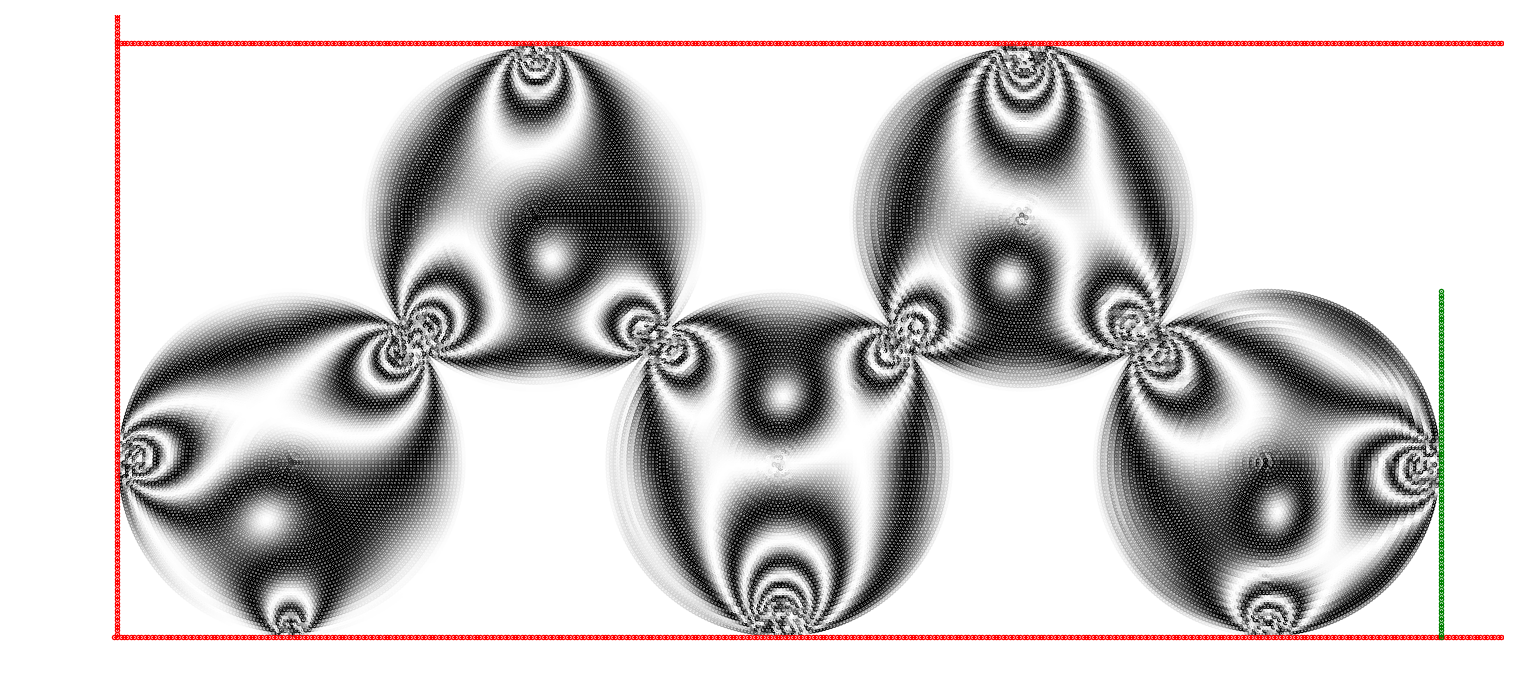
\includegraphics[width=0.8\textwidth]{figures/csph/figures/de_2021_stress_wave_in_granular_material_part_2/case_mohseni/time0}
    \subcaption{}\label{fig:de-stress-wave-current}
  \end{subfigure}
  \caption{Stress fringes of the granular discs from (a) experiment
    \citep{guilkey2001improved}, (b) TLMPM \citep{de2021modelling} (c) Current work}
\label{fig:de-stress-wave-compare}
\end{figure}

% \include{chapter_synopsis/implementation_details}
\chapter{Fluid-structure interaction}
\label{sec:fsi}
We model FSI with the developed CTVF scheme. This is advantageous since it can
eliminate the tensile instability issue in solid dynamics and ensure a homogeneous
particle distribution in fluids without any additional artificial stress terms.
We model FSI by the CTVF method, where both fluids and solid phases are modeled
using CTVF alone, while the interaction is modeled using a dummy particle
approach \citep{Adami2012}. We additionally consider the force acting on fluid
particles due to the interaction with the structure in the momentum equation. A
similar modification is carried out to the solid particle momentum equation as
well. The force is computed using a dummy particle approach of
\textcite{Adami2012}.


We study the deformation of the elastic plate due to the impact of water from a
dam break. The material properties of the elastic plate with a density of $2500$
kgm\textsuperscript{-3}, Young's modulus of $10^6$ Pa, and a Poisson ratio of
$0$. The material properties of the fluid are a density of 1000
kgm\textsuperscript{-3}, with no dynamic viscosity. In
\cref{fig:dam-breaking-onto-plate-snapshot}, we show the schematic of the
elastic dam break, and the deformed structure with fluid rise at a time instant.
\Cref{fig:water-impact-plate-deflection-quantitative} compares displacement of
the tip of the structure simulated with the current solver to other numerical
implementations. The current solver results are close to the other numerical
models.
\begin{figure}[tpb]
    \centering
  \begin{subfigure}{0.48\textwidth}
    \centering
    \includegraphics[scale=0.3]{images/fsi/images/sun_2019_dam_breaking_flow_impacting_an_elastic_plate/schematic}
    \caption{}
  \end{subfigure}
  \begin{subfigure}{0.48\textwidth}
    \centering
        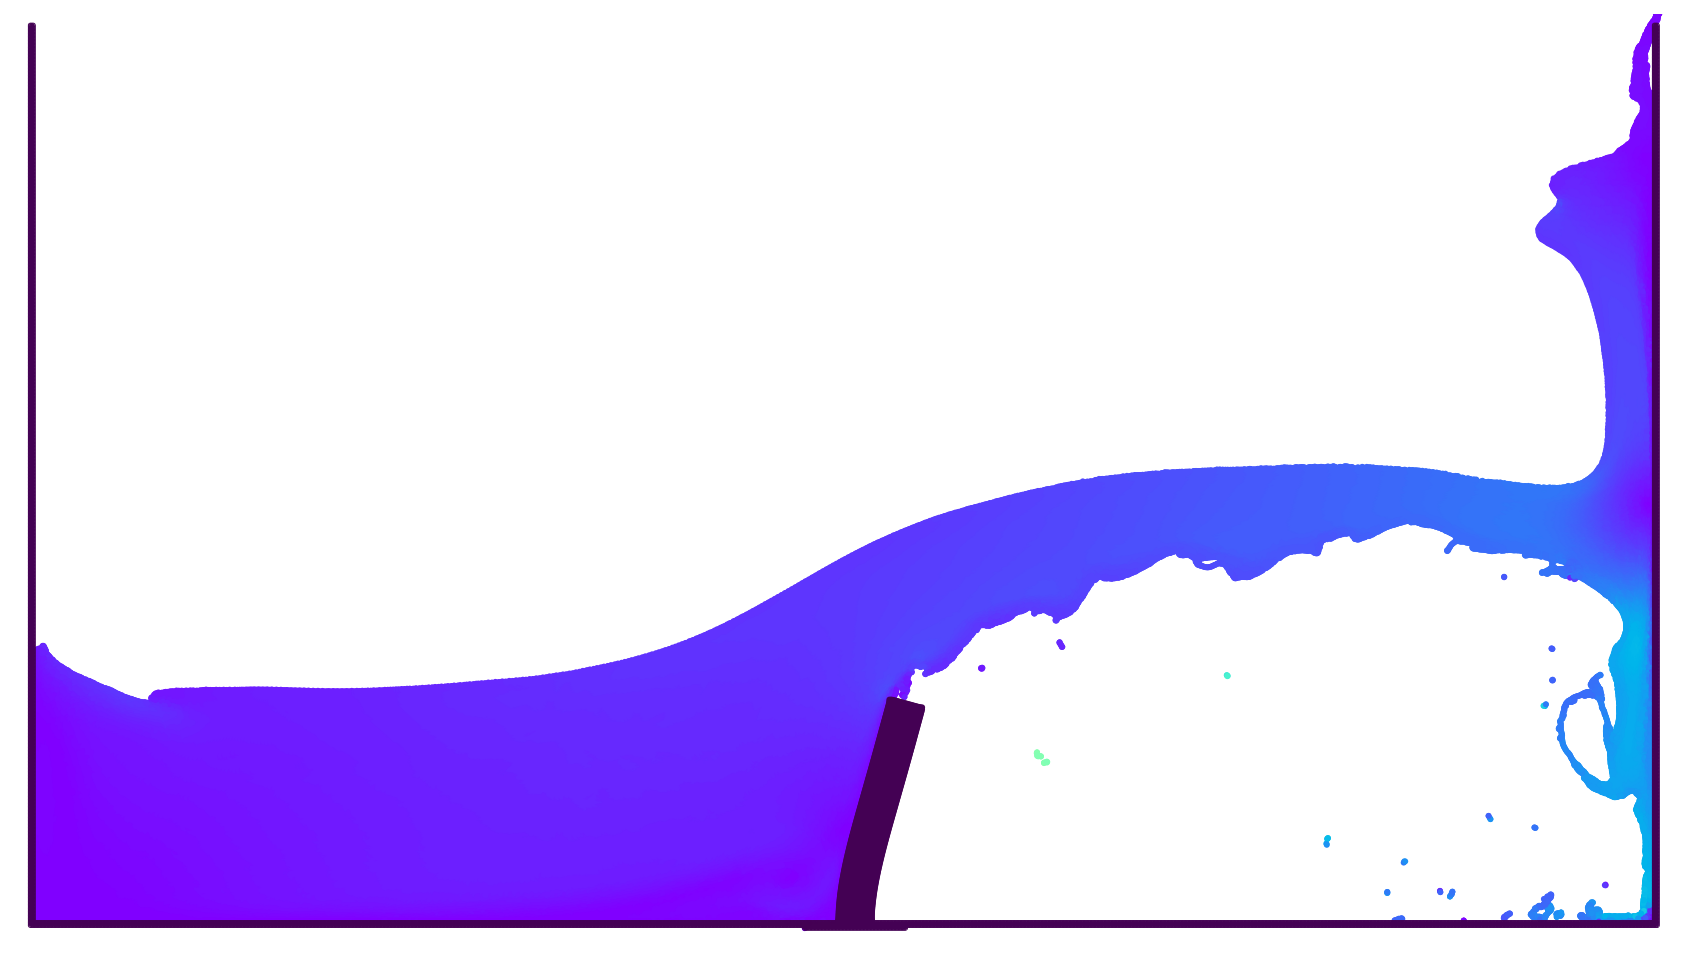
\includegraphics[scale=0.4]{figures/fsi/figures/sun_2019_dam_breaking_flow_impacting_an_elastic_plate/snap_t_2.png}
        \caption{}
  \end{subfigure}
    \caption
    { (a) Schematic of dam break flow over an elastic obstacle. (b) Snapshot of
      the deformed structure obstructing the fluid. }
    \label{fig:dam-breaking-onto-plate-snapshot}
\end{figure}
\begin{figure}[tpb]
  \centering
  \includegraphics[scale=0.45]{figures/fsi/figures/sun_2019_dam_breaking_flow_impacting_an_elastic_plate/x_amplitude}
  \caption{Time histories of horizontal displacement of the free end of the
    elastic structure compared against the numerical results of
    \citep{sun2019fully,bogaers2016evaluation}- Dam breaking flow impacting an
    elastic plate.}
\label{fig:water-impact-plate-deflection-quantitative}
\end{figure}
We have found that, the coupled CTVF solver is able to predict the deformation of the elastic
structure under hydrodynamics loads accurately.

\FloatBarrier%
\chapter{Rigid-fluid coupling}
\label{chap:rfc}
We model the dynamics of rigid bodies in fluid flow and the coupled behavior of
fluid and rigid bodies. Transport of arbitrarily shaped rigid bodies in fluid
flows is a common phenomenon that occurs widely in nature. We couple CTVF with
DEM to handle the rigid fluid coupling problems. The fluid phase is modeled
using a corrected transport velocity formulation. CTVF provides smooth pressure
distribution with EDAC formulation and homogeneous particle distribution,
resulting in accurate fluid modeling. Rigid-rigid interactions are modeled with
DEM. The interaction between the fluid phase and rigid bodies is handled using
the dummy particle approach.

We demonstrate the CTVF-DEM model by simulating sliding of a rigid cube on a
frictional inclined plane, and rising of a cylinder in a
hydrostatic tank.


\FloatBarrier%
\section{Rigid body sliding down an inclined plane}
\label{sec:rigid-body-sliding}
The rigid body of length $0.1$ m, height
$0.1$ m, is allowed to slide on a frictional surface which is at an angle
$\frac{\pi}{3}$. The schematic is shown is \cref{fig:rigid_body_sliding}. A
density of $2000$ kg\,m\textsuperscript{-3} is used for the body.
\begin{figure}[!htpb]
  \centering
  \includegraphics[width=0.4\textwidth]{images/rfc/images/rigid_body_sliding/schematic}
  \caption{Schematic of a square body sliding down an inclined plane under gravity.}
\label{fig:rigid_body_sliding}
\end{figure}
We have considered three different friction coefficients, $\mu=0.2$, $0.3$, and
$0.6$. From the analytical solution, when the friction coefficient is greater
than $\tan(\frac{\pi}{3})$, we have no slip condition and the body doesn't
slide.

\Cref{fig:results-solid-sliding-velocity-vs-time-2d} shows a evolution of
velocity of the center of mass of the rigid body for different frictional
coefficients against the analytical solution. From
\cref{fig:results-solid-sliding-velocity-vs-time-2d} we can see that the current
solver has an excellent match with the analytical solution and covers all the
regimes of the sliding case.
\begin{figure}[!htpb]
  \centering
  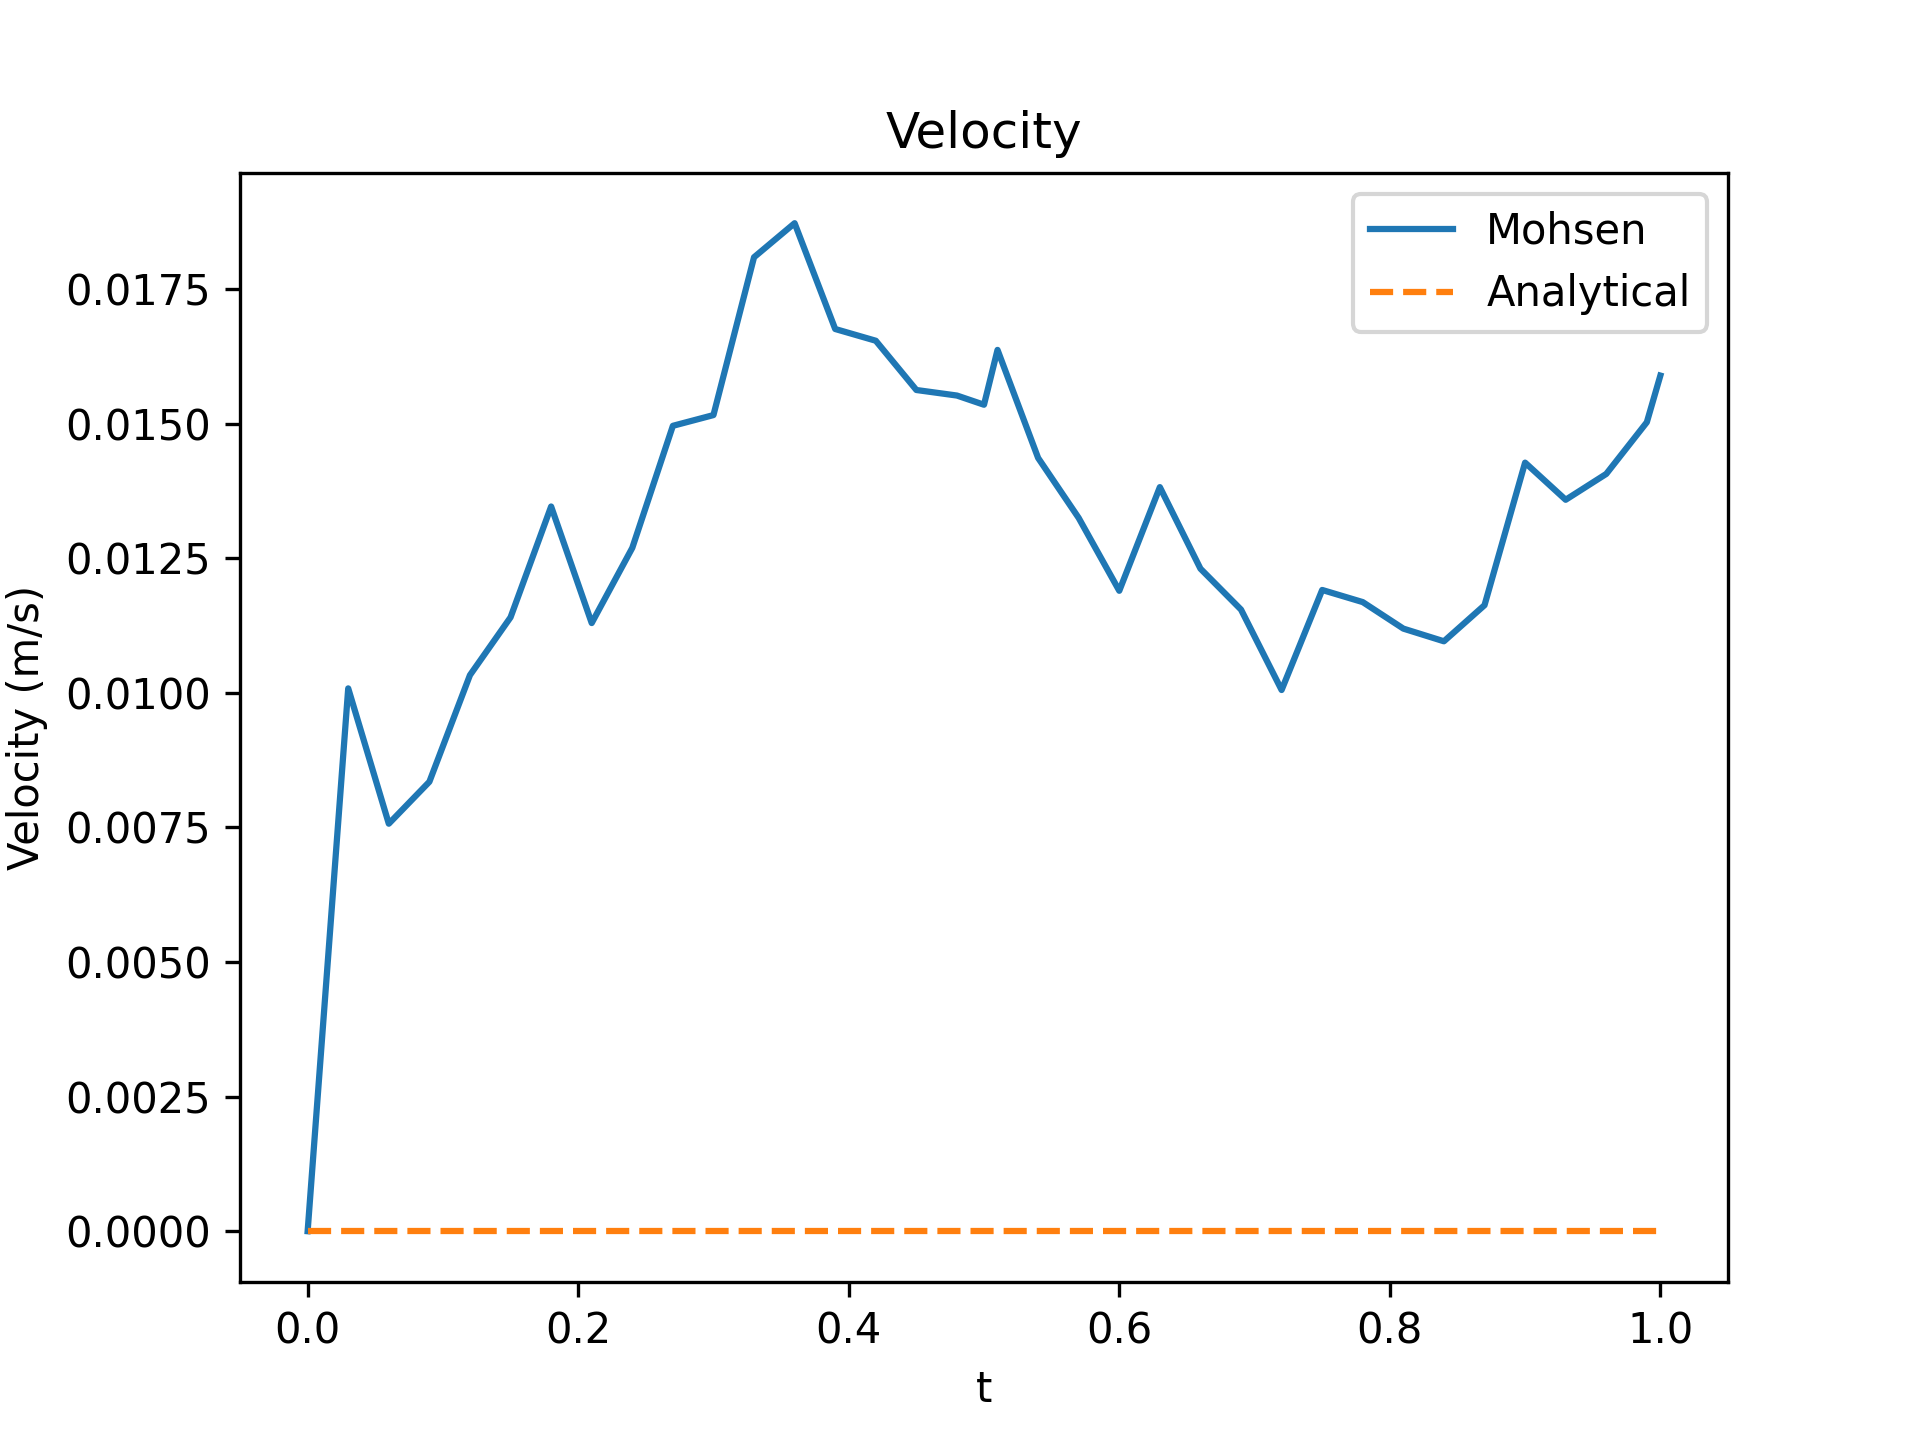
\includegraphics[width=0.6\textwidth]{figures/rfc/figures/mohseni_2021_free_sliding_on_a_slope_2d/velocity_vs_time}
  \caption{Variation of the velocity of the rigid body with time for different
    friction coefficients. Present result is compared against the analytical
    result.}
\label{fig:results-solid-sliding-velocity-vs-time-2d}
\end{figure}


\FloatBarrier%
\section{Cylinder rising in a hydrostatic tank}
\label{sec:water-entry-sphere}
% https://www.sciencedirect.com/science/article/pii/S0997754621001412#fig2
We study the behavior of a circular cylinder of density $500$
kg\,m\textsuperscript{-3} immersed in a hydrostatic tank under gravity. Since
the density of the solid body is half of the fluid, the body will be half afloat
while coming to rest. \Cref{fig:snapshots-rising-solid-in-water} presents
snapshot of a rising cylinder at time $t=15$ s and time variation of the center
of mass with time. As can be seen from the figure, since the density of the
cylinders is 500 kg\,m\textsuperscript{-3} the cylinder floats at half of its
diameter.
\begin{figure}[!htpb]
  \centering
    \includegraphics[width=0.4\textwidth]{images/rfc/images/water_entry_of_sphere/schematic}
  \caption{The schematic of an immersed cylinder in a hydrostatic tank.}
\label{fig:raising-falling-solid-in-water}
\end{figure}

\begin{figure}[!htpb]
  \centering
  \begin{subfigure}{0.48\textwidth}
    \centering
    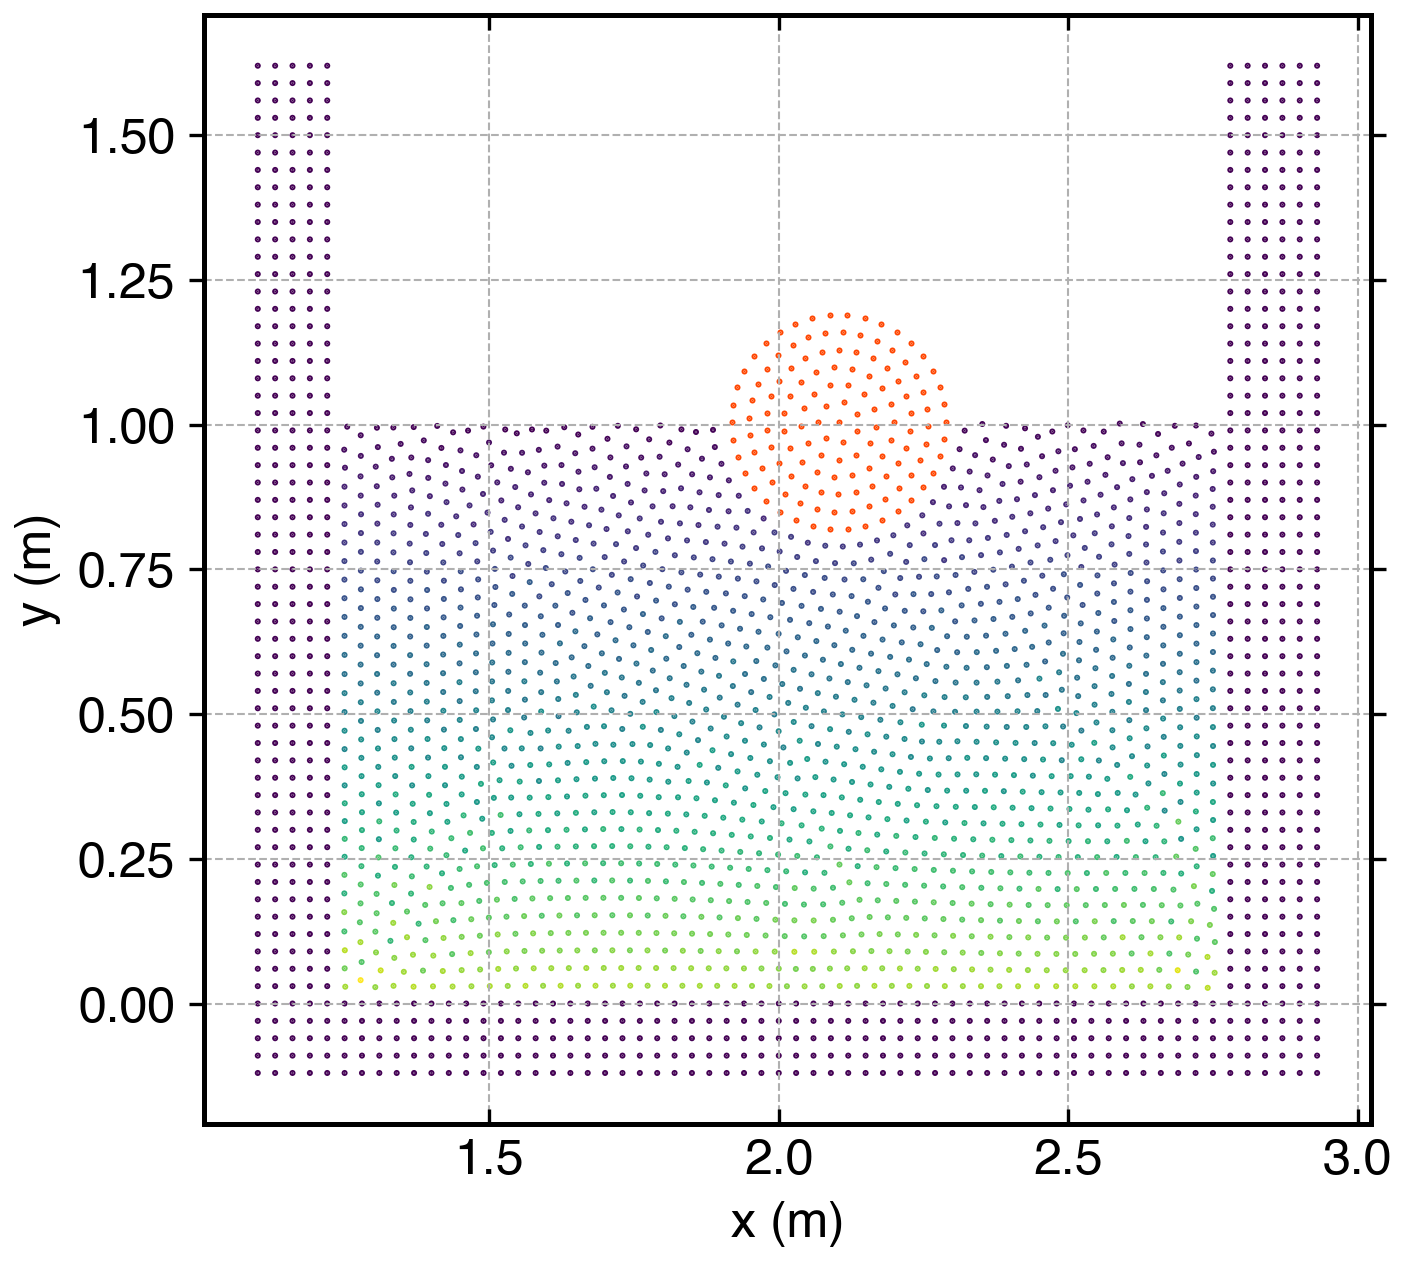
\includegraphics[width=1.0\textwidth]{figures/rfc/figures/dinesh_2022_body_in_hs_tank_2d/time11}
  \end{subfigure}
  %
  \begin{subfigure}{0.48\textwidth}
    \centering
    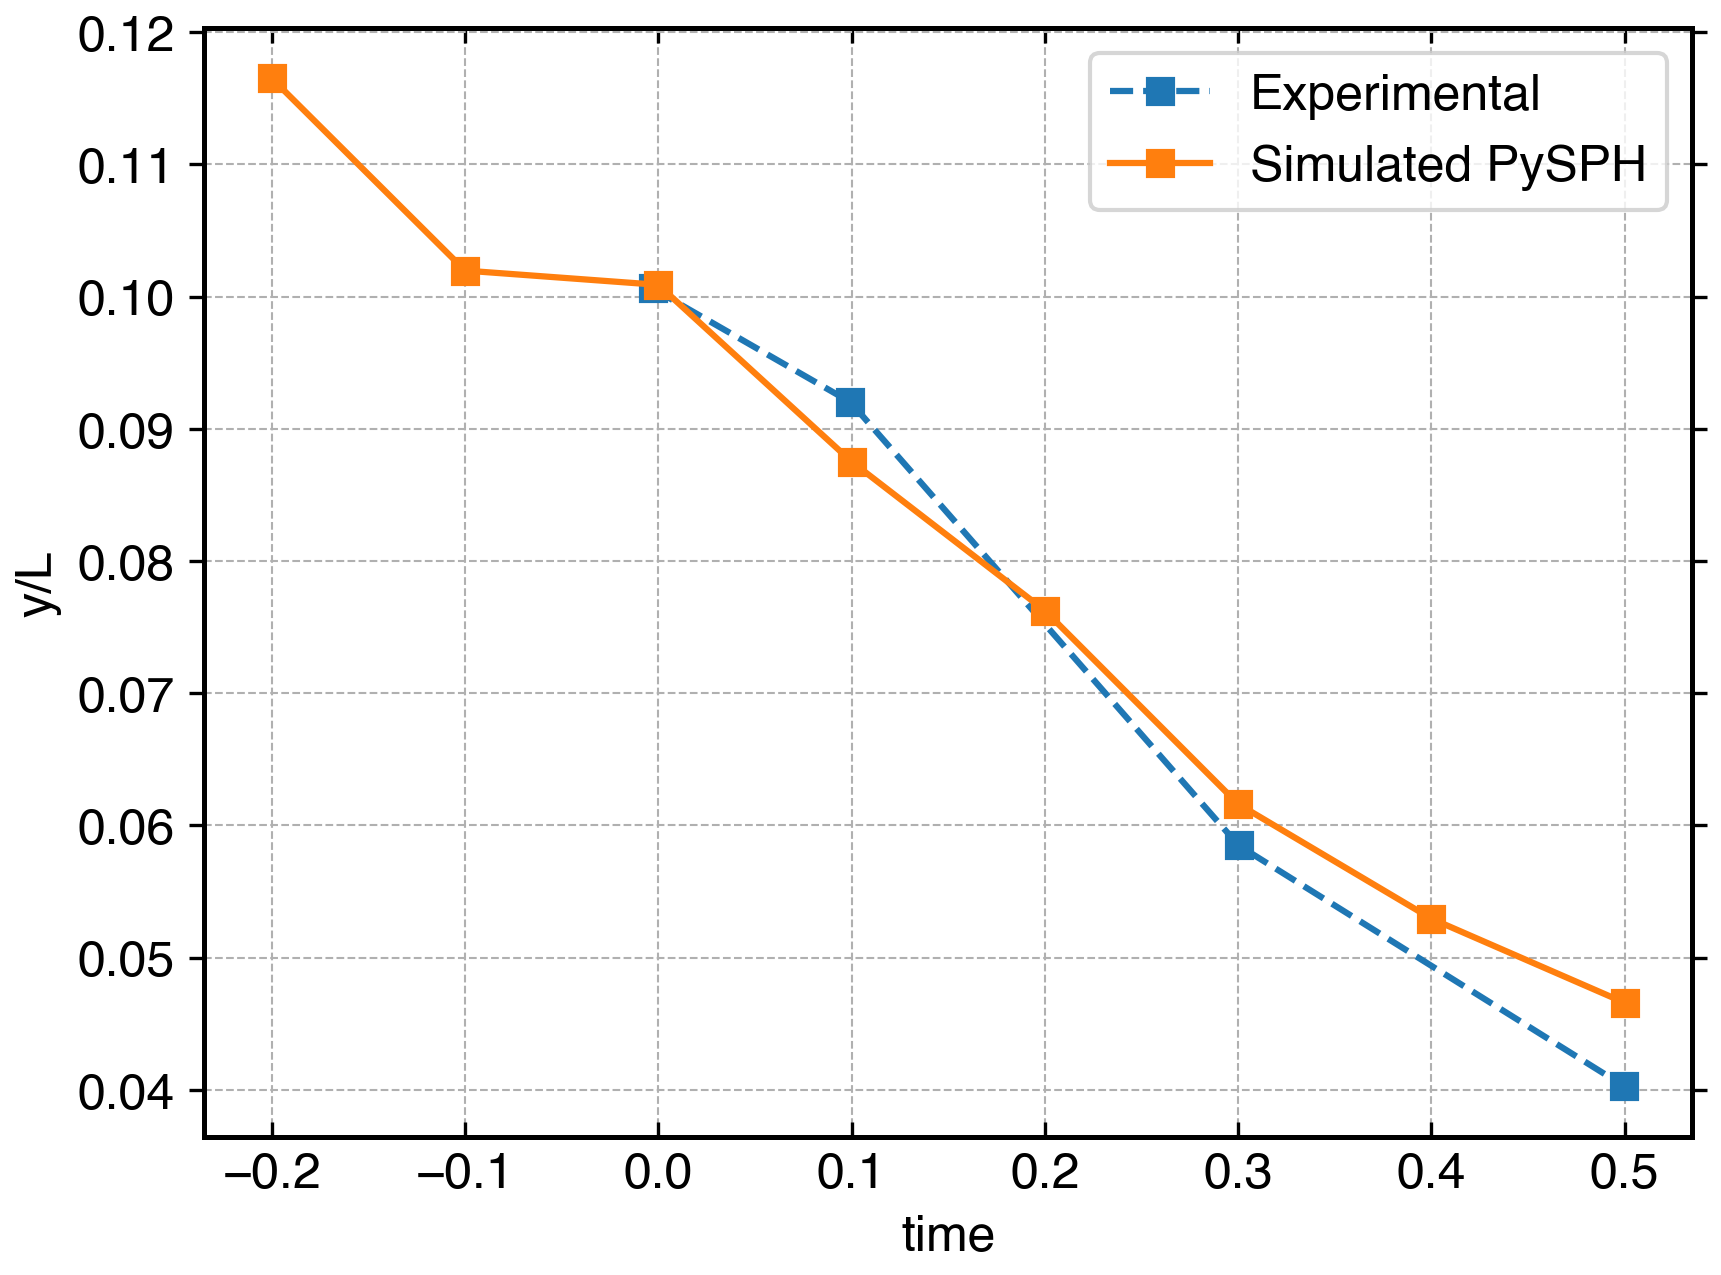
\includegraphics[width=1.0\textwidth]{figures/rfc/figures/dinesh_2022_body_in_hs_tank_2d/ycom}
  \end{subfigure}
  \caption{
    On the left, a snapshot at $t=15$ s is shown. On the right,
    time variation of the center of mass is shown.}
\label{fig:snapshots-rising-solid-in-water}
\end{figure}

\FloatBarrier%
\chapter{Erosion}
\label{chap:erosion}
We develop a numerical implementation to study the solid particle erosion of a
ductile target. We follow the numerical model proposed in
\citep{dong2016smoothed}. We utilize the CTVF to model the elastic behavior of
the ductile target, while the collision between the rigid bodies, elastic bodies
to modeled using DEM. We extend the developed numerical method to handle plastic
using a Johnson-Cook constitutive law. The objective of this work is to develop
an open-source framework to handle solid-particle erosion in two and three
dimensions. The solver should handle erosion of the target due to multiple
impacting particles. Here, The impacting particles may be interacting
themselves.


% ====================================================================================
% ====================================================================================
\FloatBarrier%
\section{Solid-particle erosion due to multiple square particles: with no self
  interaction}
\label{sec:res:mpe-2}

\Cref{fig:mpe-2-full} shows the snapshots for computational model 2. The target
and the body are discretized into $12708$ particles in the current case. From
\cref{fig:mpe-2-full,fig:mpe-2-border}, we can see that the both computational
models result in same erosion of the target, which is verified qualitatively by
comparing the eroded regions of of the target. For a quantitative validation, we
compare the y component of the center of mass of the bottom square particle with
time, when simulated using both the models in \cref{fig:mpe-2-ycom-vs-t}. From
\cref{fig:mpe-2-ycom-vs-t}, we can see that both the computational models give
the same result. Though both the models result in same erosion of the target,
however, computational model 1 is $2.3$ times faster than computational model 2.
This is due to boundary particle representation in the 1st model. A clearer
description is shown in \cref{table:mpe-2-time-comparison}.
\begin{figure}[!htpb]
  \centering
  \begin{subfigure}{0.48\textwidth}
    \centering
    \includegraphics[width=\textwidth]{figures/erosion/figures/multi_body_erosion_example_2/all_particles_no_self_intersection/all_bodies_time0.pdf}
    \subcaption{}
    \label{fig:mpe-2-full-a}
  \end{subfigure}
  \begin{subfigure}{0.48\textwidth}
    \centering
    \includegraphics[width=\textwidth]{figures/erosion/figures/multi_body_erosion_example_2/all_particles_no_self_intersection/all_bodies_time1.pdf}
    \subcaption{}
    \label{fig:mpe-2-full-b}
  \end{subfigure}
  \caption{Erosion of a ductile target due to the impact of two non-interacting
    square particles with computational model 2.}
\label{fig:mpe-2-full}
\end{figure}

% ====================================================================================
% ====================================================================================
\FloatBarrier%
\section{Solid-particle erosion due to multiple square particles: with
  self interaction}
\label{sec:erosion-multiple-impact-self-interact}

\Cref{fig:mpe-1-border} shows the snapshot of the target during the impact for
the computational model 1. \Cref{fig:mpe-1-border-a} shows the penetration of
body $1$ into the ductile target, and initial impact of the body $2$ with body
$1$. \Cref{fig:mpe-1-border-b} shows the snapshot after body $1$ loses the
contact with the target. \Cref{fig:mpe-4-border} shows the snapshot of the
target during the impact for the computational model 1 with a single square
particle. From \cref{fig:mpe-4-border}, we can see that the impacting body
erodes the target symmetrically and after losing contact it moves away from the
away without acquiring a rotation. However, for the two square particle impact
case, the material is eroded more from the right side, this is due to the second
square particle impact, this can be seen in \cref{fig:mpe-1-border}.

We repeat the same experiment with computational model 2. The erosion of the
ductile solid with computational model 2 is shown in \cref{fig:mpe-1-full}. From
\cref{fig:mpe-1-full,fig:mpe-1-border}, we can see that both the computational
models results in same erosion pattern. For quantitatively validation for the
similarity, we plot center of mass of the 1st body with time in
\cref{fig:mpe-1-ycom-vs-t}. From \cref{fig:mpe-1-ycom-vs-t}, we can see that
both 1 behaves same in both the computational models. The performance comparison
of the proposed computational models are shown in
\cref{table:mpe-1-time-comparison}.
\begin{figure}[!htpb]
  \centering
  \begin{subfigure}{0.48\textwidth}
    \centering
    \includegraphics[width=\textwidth]{figures/erosion/figures/multi_body_erosion_example_1/all_particles_self_intersection/all_bodies_time0.pdf}
    \subcaption{}
    \label{fig:mpe-1-full-a}
  \end{subfigure}
  \begin{subfigure}{0.48\textwidth}
    \centering
    \includegraphics[width=\textwidth]{figures/erosion/figures/multi_body_erosion_example_1/all_particles_self_intersection/all_bodies_time1.pdf}
    \subcaption{}
    \label{fig:mpe-1-full-b}
  \end{subfigure}
  \caption{Erosion of a ductile target due to the impact of two interacting
    square particles with computational model 2.}
\label{fig:mpe-1-full}
\end{figure}

\begin{table}[!htpb]
\centering
\begin{tabular}{c c c c c}
  \hline
  Model & No. particles & Time taken & Scale up  \\
  \hline
  Computational model 1 & $8476$ & $239.36$ sec & $1.956$ \\
  Computational model 2 & $12708$ & $468.21$ sec & 1 \\
\end{tabular}
\caption{CPU time comparison of computational model 1 and computational model 2
  for solid particle erosion for interacting particles.}
\label{table:mpe-1-time-comparison}
\end{table}
The demonstrated test cases show that the developed software can handle the
modeling erosion of a body in 2 and 3 dimensions. Further, we verified that the
representation of projectiles with border particles reduces the time of
computation. We established the current framework for handling erosion due to
multiple particle impacts.

\input{chapter_synopsis/conclusions_synopsis}

\backmatter%

\begingroup
\sloppy
\printbibliography[notcategory=fullcited]%
\endgroup

%%%
\listofpublications

\subsection*{Journal proceedings}

\begin{itemize}
\item \textbf{Dinesh Adepu} and Prabhu Ramachandran. ``\textbf{A corrected transport-velocity
  formulation for fluid and structural mechanics with SPH}''. in : arXiv preprint
  arXiv:2106.00756 (2021). Under review.
\item \textbf{Dinesh Adepu} and Prabhu Ramachandran. ``\textbf{Improved collision handling of
  elastic solids in SPH using a contact force model}''. in : Engineering Archive
  preprint (Aug. 2022). Under review.
\item Prabhu Ramachandran, Aditya Bhosale, Kunal Puri, Pawan Negi, Abhinav Muta,
  \textbf{Adepu Dinesh}, Dileep Menon, Rahul Govind, Suraj Sanka, Amal S. Sebastian,
  Ananyo Sen, Rohan Kaushik, Anshuman Kumar, Vikas Kurapati, Mrinalgouda Patil,
  Deep Tavker, Pankaj Pandey, Chandrashekhar Kaushik, Arkopal Dutt, and Arpit
  Agarwal. 2021. ``\textbf{PySPH : A Python-based Framework for Smoothed Particle
  Hydrodynamics}''. ACM Trans. Math. Softw. 47, 4, Article 34 (December 2021), 38
  pages.
\end{itemize}


\subsection*{Conference proceedings}
\label{sec:conf-proc}
\begin{itemize}
\item Dinesh Adepu and Prabhu Ramachandran. "Fluid-Structure Interaction with an
  Updated Lagrangian Smoothed Particle Hy- drodynamics". in : 9th International
  and 49th National Conference of Fluid Mechanics and Fluid Power (FMFP-2022)
  (Dec. 2022)
\end{itemize}




%%======================================================================
%%% Local Variables:
%%% mode: latex
%%% TeX-master: "../mainrep"
%%% End:


\end{document}

%%% Local Variables:
%%% mode: latex
%%% TeX-master: t
%%% End:
